%\documentclass[hyperref={pdfpagelabels=false},slidetop,9pt]{beamer}
\documentclass[slidetop,8pt]{beamer}
\usepackage[T1]{fontenc}
\usepackage[utf8]{inputenc}
\newcommand{\nom}{Porte conteneur}
\newcommand{\sequence}{03}
\newcommand{\num}{04}
\newcommand{\type}{TD}
\newcommand{\descrip}{Résolution d'un problème en utilisant des méthodes algorithmiques}
\newcommand{\competences}{Alt-C3: Concevoir un algorithme répondant à un problème précisément posé}
\usepackage{etex}
\usepackage{tikz}
\usepackage[european]{circuitikz}
\usepackage{pgf}
\usepackage[all]{xy}
\usepackage{pgfpages}
\usepackage{graphbox}
\usepackage{pdfpages}
\usepackage[adobe-utopia]{mathdesign}
\usepackage{ifthen}
\usepackage{cancel}
\usepackage{framed}
\usepackage{subfig}
\usepackage{tabularx}
\usepackage{setspace}
\usepackage{soul}
\usepackage{schemabloc}
\usepackage{eqnarray}
\usepackage[dot, phantomtext]{dashundergaps}
\usepackage{media9}
\usepackage{multimedia}

\author{Renaud Costadoat}
\institute{Lycée Dorian}

\usepackage{multido}
\usepackage{multirow}
\usepackage{multicol} % Portions de texte en colonnes
\usepackage{flafter}%floatants après la référence

\usepackage{color}
\usepackage{xcolor}
\usepackage{colortbl}

\usepackage[gen]{eurosym}
\usepackage{tikz}
%\usepackage{pstricks,pst-node,pst-tree,pst-solides3d}
\usepackage{lmodern}
\usepackage[francais]{babel}
\usepackage{pslatex}
\usetheme{renaud}
\usepackage{times}
\usepackage{amsmath}
\usepackage{verbatim}
\usepackage{moreverb}
%\usetikzlibrary{arrows,shapes}
\usepackage{graphicx}
\usepackage{psfrag}
\usepackage{wrapfig}
\usepackage{etoolbox}

\definecolor{gris25}{gray}{0.75}
\definecolor{bleu}{RGB}{18,33,98}
\definecolor{bleuf}{RGB}{42,94,171}
\definecolor{bleuc}{RGB}{231,239,247}
\definecolor{rougef}{RGB}{185,18,27}
\definecolor{rougec}{RGB}{255,188,204}%255,230,231
\definecolor{vertf}{RGB}{103,126,82}
\definecolor{vertc}{RGB}{220,255,191}

\setlength\parindent{24pt}
\parskip 7.2pt
\parindent 8pt

\newenvironment{rem}[1][\hsize]%
{%
    \def\FrameCommand
   {%
\rotatebox{90}{\textit{\textsf{Remarque}}} 
       {\color{bleuf}\vrule width 3pt}%
       \hspace{0pt}%must no space.
       \fboxsep=\FrameSep\colorbox{bleuc}%
  }%
    \MakeFramed{\hsize#1\advance\hsize-\width\FrameRestore}%
}%
{\endMakeFramed}%


\newenvironment{savoir}[1][\hsize]%
{%
    \def\FrameCommand
    {%
\rotatebox{90}{\textit{\textsf{Savoir}}} 
        {\color{bleuf}\vrule width 3pt}%
        \hspace{0pt}%must no space.
        \fboxsep=\FrameSep\colorbox{bleuc}%
    }%
    \MakeFramed{\hsize#1\advance\hsize-\width\FrameRestore}%
}%
{\endMakeFramed}%

\newenvironment{prob}[1][\hsize]%
{%
    \def\FrameCommand%
    {%
\rotatebox{90}{\textit{\textsf{Problématique}}} 
        {\color{rougef}\vrule width 3pt}%
        \hspace{0pt}%must no space.
        \fboxsep=\FrameSep\colorbox{rougec}%
    }%
    \MakeFramed{\hsize#1\advance\hsize-\width\FrameRestore}%
}%
{\endMakeFramed}%

\newenvironment{obj}[1][\hsize]%
{%
    \def\FrameCommand%
    {%
\rotatebox{90}{\textit{\textsf{Objectif}}} 
        {\color{vertf}\vrule width 3pt}%
        \hspace{0pt}%must no space.
        \fboxsep=\FrameSep\colorbox{vertc}%
    }%
    \MakeFramed{\hsize#1\advance\hsize-\width\FrameRestore}%
}%
{\endMakeFramed}%

\newenvironment{defi}[1][\hsize]%
{%
    \def\FrameCommand%
    {%
\rotatebox{90}{\textit{\textsf{Definition}}} 
        {\color{bleuf}\vrule width 3pt}%
        \hspace{0pt}%must no space.
        \fboxsep=\FrameSep\colorbox{rougec}%
    }%
    \MakeFramed{\hsize#1\advance\hsize-\width\FrameRestore}%
}%
{\endMakeFramed}%


\newenvironment{hypo}[1][\hsize]%
{%
    \def\FrameCommand%
    {%
\rotatebox{90}{\textit{\textsf{Hypothèse\\}}} 
        {\color{bleuf}\vrule width 3pt}%
        \hspace{0pt}%must no space.
        \fboxsep=\FrameSep\colorbox{bleuc}%
    }%
    \MakeFramed{\hsize#1\advance\hsize-\width\FrameRestore}%
}%
{\endMakeFramed}%


\newenvironment{prop}[1][\hsize]%
{%
    \def\FrameCommand%
    {%
\rotatebox{90}{\textit{\textsf{Propriété}}} 
        {\color{bleuf}\vrule width 3pt}%
        \hspace{0pt}%must no space.
        \fboxsep=\FrameSep\colorbox{bleuc}%
    }%
    \MakeFramed{\hsize#1\advance\hsize-\width\FrameRestore}%
}%
{\endMakeFramed}%

\newenvironment{props}[1][\hsize]%
{%
    \def\FrameCommand%
    {%
\rotatebox{90}{\textit{\textsf{Propriétés}}} 
        {\color{bleuf}\vrule width 3pt}%
        \hspace{0pt}%must no space.
        \fboxsep=\FrameSep\colorbox{bleuc}%
    }%
    \MakeFramed{\hsize#1\advance\hsize-\width\FrameRestore}%
}%
{\endMakeFramed}%

\newenvironment{exemple}[1][\hsize]%
{%
    \def\FrameCommand%
    {%
\rotatebox{90}{\textit{\textsf{Exemple}}} 
        {\color{vertf}\vrule width 3pt}%
        \hspace{0pt}%must no space.
        \fboxsep=\FrameSep\colorbox{vertc}%
    }%
    \MakeFramed{\hsize#1\advance\hsize-\width\FrameRestore}%
}%
{\endMakeFramed}%

\newenvironment{resultat}[1][\hsize]%
{%
    \def\FrameCommand%
    {%
\rotatebox{90}{\textit{\textsf{Resultat}}} 
        {\color{rougef}\vrule width 3pt}%
%        {\color{bleuf}\vrule width 3pt}%
        \hspace{0pt}%must no space.
        \fboxsep=\FrameSep\colorbox{rougec}%
    }%
    \MakeFramed{\hsize#1\advance\hsize-\width\FrameRestore}%
}%
{\endMakeFramed}%

\newenvironment{methode}[1][\hsize]%
{%
    \def\FrameCommand%
    {%
\rotatebox{90}{\textit{\textsf{Méthode\\}}} 
        {\color{rougef}\vrule width 3pt}%
        \hspace{0pt}%must no space.
        \fboxsep=\FrameSep\colorbox{rougec}%
    }%
    \MakeFramed{\hsize#1\advance\hsize-\width\FrameRestore}%
}%
{\endMakeFramed}%

\newenvironment{theo}[1][\hsize]%
{%
    \def\FrameCommand%
    {%
\rotatebox{90}{\textit{\textsf{Théorème\\}}} 
        {\color{rougef}\vrule width 3pt}%
        \hspace{0pt}%must no space.
        \fboxsep=\FrameSep\colorbox{rougec}%
    }%
    \MakeFramed{\hsize#1\advance\hsize-\width\FrameRestore}%
}%
{\endMakeFramed}%

\newenvironment{warn}[1][\hsize]%
{%
    \def\FrameCommand%
    {%
\rotatebox{90}{\textit{\textsf{Attention\\}}} 
        {\color{rougef}\vrule width 3pt}%
        \hspace{0pt}%must no space.
        \fboxsep=\FrameSep\colorbox{rougec}%
    }%
    \MakeFramed{\hsize#1\advance\hsize-\width\FrameRestore}%
}%
{\endMakeFramed}%

% \usepackage{pstricks}
%\usepackage{minitoc}
% \setcounter{minitocdepth}{4}

\setcounter{tocdepth}{2}

% \mtcselectlanguage{french} 

%\usepackage{draftcopy}% "Brouillon"
% \usepackage{floatflt}
\usepackage{psfrag}
%\usepackage{listings} % Permet d'insérer du code de programmation
\renewcommand{\baselinestretch}{1.2}

% Changer la numérotation des figures :
% ------------------------------------
% \makeatletter
% \renewcommand{\thefigure}{\ifnum \c@section>\z@ \thesection.\fi
%  \@arabic\c@figure}
% \@addtoreset{figure}{section}
% \makeatother
 


%%%%%%%%%%%%
% Définition des vecteurs %
%%%%%%%%%%%%
 \newcommand{\vect}[1]{\overrightarrow{#1}}

%%%%%%%%%%%%
% Définition des torseusr %
%%%%%%%%%%%%

 \newcommand{\torseur}[1]{%
\left\{{#1}\right\}
}

\newcommand{\torseurcin}[3]{%
\left\{\mathcal{#1} \left(#2/#3 \right) \right\}
}

\newcommand{\torseurstat}[3]{%
\left\{\mathcal{#1} \left(#2\rightarrow #3 \right) \right\}
}

 \newcommand{\torseurc}[8]{%
%\left\{#1 \right\}=
\left\{
{#1}
\right\}
 = 
\left\{%
\begin{array}{cc}%
{#2} & {#5}\\%
{#3} & {#6}\\%
{#4} & {#7}\\%
\end{array}%
\right\}_{#8}%
}

 \newcommand{\torseurcol}[7]{
\left\{%
\begin{array}{cc}%
{#1} & {#4}\\%
{#2} & {#5}\\%
{#3} & {#6}\\%
\end{array}%
\right\}_{#7}%
}

 \newcommand{\torseurl}[3]{%
%\left\{\mathcal{#1}\right\}_{#2}=%
\left\{%
\begin{array}{l}%
{#1} \\%
{#2} %
\end{array}%
\right\}_{#3}%
}

 \newcommand{\vectv}[3]{%
\vect{V\left( {#1} \in {#2}/{#3}\right)}
}


\newcommand{\vectf}[2]{%
\vect{R\left( {#1} \rightarrow {#2}\right)}
}

\newcommand{\vectm}[3]{%
\vect{\mathcal{M}\left( {#1}, {#2} \rightarrow {#3}\right)}
}


 \newcommand{\vectg}[3]{%
\vect{\Gamma \left( {#1} \in {#2}/{#3}\right)}
}

 \newcommand{\vecto}[2]{%
\vect{\Omega\left( {#1}/{#2}\right)}
}

\newcommand{\reponse}[1][4]
{
\multido{}{#1}
{
\begin{center}
\makebox[0.9\linewidth]{\dotfill} \end{center}
}}


% }$$\left\{\mathcal{#1} \right\}_{#2} =%
% \left\{%
% \begin{array}{c}%
%  #3 \\%
%  #4 %
% \end{array}%
% \right\}_{#5}}


%  ------------------------------------------
% | Modification du formatage des sections : | 
%  ------------------------------------------

% Grands titres :
% ---------------

\newcommand{\titre}[1]{%
\begin{center}
      \bigskip
      \rule{\textwidth}{1pt}
      \par\vspace{0.1cm}
      
      \textbf{\large #1}
      \par\rule{\textwidth}{1pt}
    \end{center}
    \bigskip
  }

% Supprime le numéro du chapitre dans la numérotation des sections:
% -----------------------------------------------------------------
\makeatletter
\renewcommand{\thesection}{\@arabic\c@section}
\makeatother


% \titleformat{\chapter}[display]
% {\normalfont\Large\filcenter}
% {}
% {1pc}
% {\titlerule[1pt]
%   \vspace{1pc}%
%   \Huge}[\vspace{1ex}%
% \titlerule]


%%%% Chapitres Comme PY Pechard %%%%%%%%%
% numéro du chapitre
\DeclareFixedFont{\chapnumfont}{OT1}{phv}{b}{n}{80pt}
% pour le mot « Chapitre »
\DeclareFixedFont{\chapchapfont}{OT1}{phv}{m}{it}{40pt}
% pour le titre
\DeclareFixedFont{\chaptitfont}{T1}{phv}{b}{n}{25pt}

\definecolor{gris}{gray}{0.75}
\setbeamertemplate{section in toc}[sections numbered]

\newlength{\RoundedBoxWidth}
\newsavebox{\GrayRoundedBox}
\newenvironment{GrayBox}[1][\dimexpr\textwidth-4.5ex]%
   {\setlength{\RoundedBoxWidth}{\dimexpr#1}
    \begin{lrbox}{\GrayRoundedBox}
       \begin{minipage}{\RoundedBoxWidth}}%
   {   \end{minipage}
    \end{lrbox}
    \begin{center}
    \begin{tikzpicture}%
       \draw node[draw=bleuf,fill=bleuc,rounded corners,%
             inner sep=2ex,text width=\RoundedBoxWidth]%
             {\usebox{\GrayRoundedBox}};
    \end{tikzpicture}
    \end{center}}
    
\ifdef{\prive}{\pgfpagesuselayout{2 on 1}[a4paper,border shrink=0mm]}
\ifdef{\prive}{\setbeamertemplate{navigation symbols}{}}
\setbeamertemplate{itemize item}[ball]
%\setbeamertemplate{blocks}[rounded]%[shadow=true]
\setbeamercolor{block title}{fg=white,bg=grisf}        % titre block normal 
\setbeamercolor{block body}{fg=grisf,bg=grisc!50}      % corps block normal
\setbeamercolor{block body alerted}{fg=white,bg=warning}   % idem pour un block alerte

\title{\nom}
\date{S\sequence \ - \type\num}

\begin{document}
\shorthandoff{:!}
\bibliographystyle{abbrvnat-fr}

\usebackgroundtemplate%
{%
    \centering
\includegraphics[width=\paperwidth]{../../img/fond2}%
}

{
\setbeamertemplate{navigation symbols}{}
\setbeamertemplate{headline}[pagetitre]
\setbeamertemplate{footline}[pagetitre]
\usebackgroundtemplate{\centering
\includegraphics[width=\paperwidth]{../../img/fond}}
\frame{\titlepage}
}



\section{Complexité} 

\begin{frame}[fragile]
\frametitle{Définition}

Il existe souvent plusieurs façons de programmer un algorithme. Ainsi, lorsque le nombre d'opérations et la taille des données d'entrée deviennent importants, deux paramètres deviennent déterminants : 
\begin{itemize}
 \item le temps d'exécution,
 \item l'occupation mémoire.
\end{itemize}

\begin{itemize}
 \item La \textbf{complexité en temps} donne le nombre d'opérations ou d'instructions effectuées lors de l'exécution d'un programme. On appelle $C_o$ le coût en temps d'une opération $o$,
 \item La \textbf{complexité en mémoire} donne le nombre d'emplacements mémoires occupés lors de l'exécution d'un
programme.
\end{itemize}

On distingue la complexité dans le pire des cas, la complexité dans le meilleure des cas, ou la complexité en moyenne.

\begin{itemize}
 \item En effet, pour un même algorithme, suivant les données à manipuler, le résultat sera déterminé plus ou moins
rapidement,
\item Généralement, on s'intéresse au cas le plus défavorable à savoir, la complexité dans le pire des cas.
\end{itemize}
\end{frame}

\begin{frame}[fragile]
\frametitle{Exemple}

Déterminer la position d'une valeur dans une liste.

\begin{minipage}[t]{0.48\linewidth}
Recherche naïve
\begin{GrayBox}[0.75\textwidth]
\begin{verbatimtab}[3]
def number_list(nb,tab):
    for i in range(len(tab)):
        if tab[i]==nb:
            return i
    return None
\end{verbatimtab}
\end{GrayBox}

Résultats:
\begin{GrayBox}[0.85\textwidth]
\begin{verbatimtab}[3]
>>> nb=25
>>> tab=range(1,100,2)
>>> number_list(nb,tab)
12
>>> number_list_dicho(nb,tab)
12
\end{verbatimtab}
\end{GrayBox}

\end{minipage}\hfill
\begin{minipage}[t]{0.48\linewidth}
Recherche par dichotomie
\begin{GrayBox}[0.85\textwidth]
\begin{verbatimtab}[3]
def number_list_dicho(nb,tab):
    g, d = 0, len(tab)-1
    while g <= d:
        m = (g + d) // 2
        if tab[m] == nb:
            return m
        if tab[m] < nb:
            g = m+1
        else:d = m-1
    return None
\end{verbatimtab}
\end{GrayBox}
\end{minipage}
\end{frame}

\begin{frame}[fragile]
\frametitle{Exemple}

Le graphe présente le nombre maximal de boucles pour trouver un nombre en fonction de la taille de la liste. La complexité en temps n'est pas la même dans les deux cas.

\begin{center}
 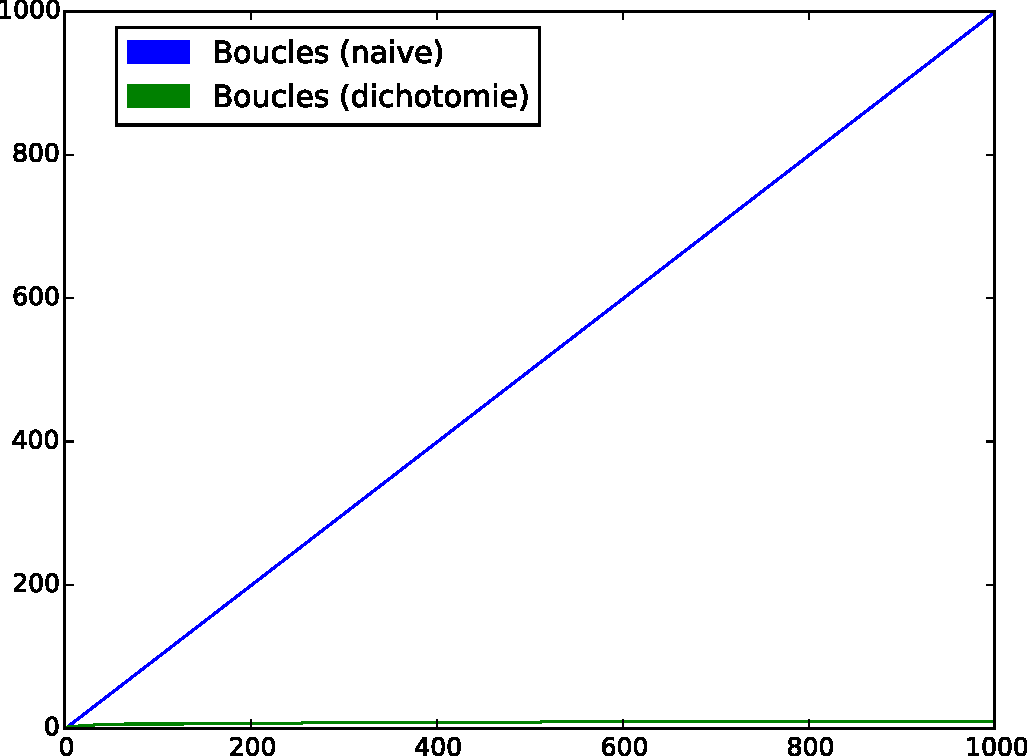
\includegraphics[width=0.65\linewidth]{img/Comp_complexite}
\end{center}

\end{frame}

\begin{frame}[fragile]
\frametitle{Coût temporel}

\begin{minipage}{0.65\linewidth}
On considère que le coût élémentaire $C_e$ correspond au coût d'une affectation, d'une comparaison ou de l'évaluation d'une opération arithmétique.
\end{minipage}\hfill
\begin{minipage}{0.3\linewidth}
\begin{GrayBox}[0.85\textwidth]
\begin{verbatimtab}[3]
>>> a=20 #(1 Ce)
>>> a<=100 #(1 Ce)
>>> a=a+1 #(2 Ce)
\end{verbatimtab}
\end{GrayBox}
\end{minipage}

\begin{minipage}{0.65\linewidth}
Pour une séquence de deux instructions de coûts respectifs $C_1$ et $C_2$, le coût total est de la séquence est de $C_1+C_2$. Le coût d'un affichage est plus important qu'un coût élémentaire.
\end{minipage}\hfill
\begin{minipage}{0.3\linewidth}
\begin{GrayBox}[0.85\textwidth]
\begin{verbatimtab}[3]
>>> a=20 #(1 Ce)
>>> print(a)  #(1 Ca)
\end{verbatimtab}
\end{GrayBox}
\end{minipage}

\begin{minipage}{0.65\linewidth}
Le coût d'un test $if\ test : inst_1 else : inst_2$ est inférieur ou égal au maximum du coût de l'instruction 1 et du coût de l'instruction 2 additionné au coût du test (coût élémentaire).
\end{minipage}\hfill
\begin{minipage}{0.3\linewidth}
\begin{GrayBox}[0.85\textwidth]
\begin{verbatimtab}[3]
>>> if x<0 :
		x=x+1
		x=x+2
	else :
		x=x+1  #(5 Ce)
\end{verbatimtab}
\end{GrayBox}
\end{minipage}
\end{frame}

\begin{frame}[fragile]
\frametitle{Calcul de coût}

Soit le programme suivant qui permet de calculer la factorielle d'un nombre.

\begin{minipage}[t]{0.48\linewidth}
\begin{GrayBox}[0.85\textwidth]
\begin{verbatimtab}[3]
def factorielle(n) :
    if  n==0:
        return 1
    else:
        i, res =1, 1
        while i<=n:
            res=res*i
            i=i+1
        return res
\end{verbatimtab}
\end{GrayBox}
\end{minipage}\hfill
\begin{minipage}[t]{0.48\linewidth}
Déterminer:
\begin{itemize}
 \item la complexité en mémoire,
 \item la complexité en temps.
\end{itemize}

\ifdef{\public}{Complexité en mémoire : $n$, $res$, $i$.\\
Complexité en temps: 
\begin{itemize}
 \item $n==0$ ($1.C_e$),
 \item $i, res =1, 1$ ($2.C_e$),
 \item $n$ fois $i<=n$, $res=res*i$, $i=i+1$ ($5.n.C_e$),
 \item $return\ res$ ($1.C_r$).
\end{itemize}}{}

\end{minipage}

\ifdef{\public}{En conséquence, la complexité en temps s'élève à :
$C_T(n)=C_e+2*Ce+n*5*Ce+Cr$, ainsi, lorsque le nombre de boucles devient important: $C_T\underset{n\rightarrow\infty}{\sim}n*5*Ce$.

Il s'agit donc d'une complexité algorithmique \textbf{linéaire}, notée O(n).}{\vspace{3cm}}
\end{frame}

\begin{frame}[fragile]
\frametitle{Calcul de coût}

Soit le programme suivant qui permet de classer une liste.

\begin{minipage}[t]{0.48\linewidth}
\begin{GrayBox}[0.85\textwidth]
\begin{verbatimtab}[3]
for i in range(0,len(tab)-1):
    min=i
    for j in range(i+1,len(tab)):
        if tab[j] < tab[min]:
            min=j
    tmp=tab[i]
    tab[i]=tab[min]
    tab[min]=tmp
print tab
\end{verbatimtab}
\end{GrayBox}
\end{minipage}\hfill
\begin{minipage}[t]{0.48\linewidth}
Déterminer:
\begin{itemize}
 \item la complexité en mémoire,
 \item la complexité en temps.
\end{itemize}

\ifdef{\public}{Ici les bornes de la boucle imbriquée dépendent de l'indice $i$. Ainsi :
\begin{itemize}
 \item au rang $1$, $C_1=C_e+(n-1)(2.Ce)+3.Ce$,
 \item au rang $2$, $C_2=C_e+(n-2)(2.Ce)+3.Ce$,
 \item au rang $i$, $C_i=C_e+(n-i)(2.Ce)+3.Ce$.
\end{itemize}}{}
\end{minipage}

\ifdef{\public}{Le coût temporel peut donc s'exprimer ainsi :

$C_T(n)=\sum\limits_{i=0}^{n-1} C_e+(n-i)(2.C_e)+3.C_e =C_e.\sum\limits_{i=0}^{n-1} 4+2.n-2.i=Ce.\left(4.n+2.n^2-2.\dfrac{n.(n-1)}{2}\right)=C_e.(5.n+n^2)$. Dans ce cas, $C_T \underset{n\rightarrow\infty}{\sim}C_e.n^2$.}{\vspace{3cm}}

\end{frame}

\begin{frame}[fragile]
\frametitle{Les types de complexités}

Par ordre de complexité croissante on a donc :
\begin{itemize}
 \item $O(1)$: algorithme s'exécutant en temps constant, quelle que soit la taille des données,
 \item $O(log(n))$: algorithme rapide (complexité logarithmique), (Exemple : recherche par dichotomie dans un
tableau trié),
 \item $O(n)$: algorithme linéaire,
 \item $O(n.log(n))$: complexité n.log(n),
 \item $O(n^2)$: complexité quadratique,
 \item $O(2^n)$: complexité exponentielle.
\end{itemize}
\end{frame}

\end{document}